\documentclass{article}
\usepackage{graphicx} % Images
\usepackage{amsmath,amsthm} % Math
\usepackage{wasysym,MnSymbol} % Greek alphabets
\usepackage{mathrsfs,amsfonts,calrsfs} % Math fonts
\usepackage{newtxtext}
\usepackage{geometry} % Formatting
\usepackage[dvipsnames,svgnames]{xcolor}
\usepackage[strict]{changepage}
\usepackage{framed}
\usepackage{cancel}
\usepackage{autobreak}
\usepackage{hyperref}

\graphicspath{ {./images/} }

\providecommand{\tightlist}{
  \setlength{\itemsep}{0pt}
  \setlength{\parskip}{0pt}}

\newcommand*\sepline{%
  \begin{center}
    \rule[1ex]{.5\textwidth}{.5pt}
  \end{center}}


%\setlength{\parindent}{0pt}% cancel indentation before every line

% right cases
\newenvironment{rcases}
  {\left.\begin{aligned}}
  {\end{aligned}\right\rbrace}

% Blue block
\definecolor{blueshade}{rgb}{0.95,0.95,1} % blue block color
\newenvironment{blueblock}{
\def\FrameCommand{
  \hspace{1pt}
    {\color{DarkBlue}
    \vrule width 2pt}
    {\color{blueshade}
    \vrule width 4pt}
  \colorbox{blueshade}
}
\MakeFramed{
  \advance
  \hsize-
  \width
  \FrameRestore}
\noindent\hspace{-4.55pt}% disable indenting first paragraph
\begin{adjustwidth}{}{7pt}
\vspace{2pt}\vspace{2pt}
}
{\vspace{2pt}\end{adjustwidth}\endMakeFramed}


% Green block
\definecolor{greenshade}{rgb}{0.90,0.99,0.91} % green block
\newenvironment{greenblock}{%
\def\FrameCommand{%
  \hspace{1pt}%
    {\color{Green}%
    \vrule width 2pt}%
    {\color{greenshade}%
    \vrule width 4pt}%
  \colorbox{greenshade}%
}%
\MakeFramed{%
  \advance%
  \hsize-%
  \width%
  \FrameRestore}%
\noindent\hspace{-4.55pt}% disable indenting first paragraph
\begin{adjustwidth}{}{7pt}%
\vspace{2pt}\vspace{2pt}%
}
{%
\vspace{2pt}\end{adjustwidth}\endMakeFramed%
}


% Red block
\definecolor{redshade}{rgb}{1.00,0.90,0.90} % red block
\newenvironment{redblock}{
\def\FrameCommand{
  \hspace{1pt}
    {\color{LightCoral}
    \vrule width 2pt}
    {\color{redshade}
    \vrule width 4pt}
  \colorbox{redshade}
}
\MakeFramed{
  \advance
  \hsize-
  \width
  \FrameRestore}
\noindent\hspace{-4.55pt}% disable indenting first paragraph
\begin{adjustwidth}{}{7pt}
\vspace{2pt}\vspace{2pt}
}
{\vspace{2pt}\end{adjustwidth}\endMakeFramed}


\newtheorem{question}{Question}
\newtheorem{note}{Note}
\newtheorem{proposition}{Proposition}
\newtheorem{lemma}{Lemma}
\newtheorem{property}{Property}

\numberwithin{equation}{section} % This makes equation numbers reflect the chapter


\title{Discussion of Migration in Economics}
\author{Victor Li}
\date{October, 2024}

\begin{document}
\maketitle



\tableofcontents
\addcontentsline{toc}{section}{Intro}
\section*{Intro}
\label{sub:intro}

Migration, one of the most dynamic forces shaping economies and societies, is a powerful lens for understanding human responses to changing economic, social, and political landscapes. Whether people move for opportunities, to escape hardships, or due to natural or policy-driven shifts, migration profoundly influences labor markets, urban development, and resource allocation across regions. Various economic theories have attempted to capture the complexities behind migration patterns, offering frameworks that explain not only why people move but also how these movements reshape economies. 

In economics, migration is analyzed not just as a population shift but as a key driver of resource allocation, labor market adjustments, and regional economic growth. Economic models focus on the incentives, barriers, and expected outcomes that influence migration, examining how people respond to wages, employment opportunities, and living standards across regions. In contrast, demographics views migration primarily as a change in population distribution, tracking shifts in age, ethnicity, and family structures without emphasizing the economic motivations and impacts. While demography tells us \textit{who} moves and \textit{where}, economics delves into \textit{why} and \textit{how} these movements reshape economies.

The diverse perspectives offered by these theories help us understand migration from multiple vantage points: from individual motivations and economic expectations to broader spatial dynamics in regional and global contexts. By weaving together these insights, economists continue to enrich our understanding of migration, shedding light on the fundamental ways in which people reshape their economic realities through movement.


% section intro (end)
% -------------------------------------------------------
% -------------------------------------------------------
% -------------------------------------------------------


\part{Optimal location choice models}


\section{Lee 1966} % (fold)
\label{sec:lee_1966}

Lee's work is known as the push-pull model.





% section lee_1966 (end)
% -------------------------------------------------------
\section{Sjaastad 1962} % (fold)
\label{sec:sjaastad_1962}

Sjaastad thinks migration is in nature an investment to human capital. He challenges the prevailing view of migration,arguing that previous research, focused primarily on the factors driving migration rates, fails to adequately address whether migration effectively corrects income disparities. Sjaastad contends that evaluating migration's efficacy requires understanding its costs and returns, both for the individual and society as a whole.

\subsection{Costs} % (fold)
\label{sub:costs}
\textbf{Money costs}
\begin{itemize}
  \item These are out-of-pocket expenses like transportation, food, and lodging associated with the move.
\end{itemize}

\textbf{Non-money costs}
\begin{itemize}
  \item Opportunity costs:These represent lost earnings from not working while moving, job searching, and learning a new job.
  \item Psychic costs:These reflect the emotional burden of leaving familiar places, people, and routines. It's important to note that psychic costs are not a resource cost to the economy and should not be factored into migration investment calculations. 
\end{itemize}
% subsection costs (end)Costs


\subsection{Returns} % (fold)
\label{sub:returns}
\textbf{Money returns}
\begin{itemize}
  \item This is the positive (or negative) change to a person’s real earnings stream resulting from the move. It could be from higher nominal wages, lower work-related costs, more favorable pricing in the new area, or some combination of all three.
\end{itemize}

\textbf{Non-money returns}
\begin{itemize}
  \item Locational preferences: These reflect the migrant's subjective valuation of features in the new location compared to the old one, like weather, pollution, or congestion.
  \item Pure consumption: This is the satisfaction (or dissatisfaction) experienced during the move itself. This is comparable to the enjoyment a student may get from being on a college campus, apart from any other benefits of their education. 
\end{itemize}

\textbf{Considerations for Estimating Returns}
\begin{itemize}
  \item Occupational Upgrading: When migration is combined with a change to a higher-paying occupation, estimating returns becomes more complex. The move, the training, and any new experience gained all factor into the person's human capital. These investments will depreciate over time, both physically and economically. 
  \item Age: The age of the migrant plays a crucial role in calculating returns.  Older migrants have less time to recoup the costs of the move and any retraining.  They likely have more job-specific experience, so changing occupations comes at a higher cost. 
\end{itemize}
% subsection returns (end)

\subsection{Private vs. Social Costs and Returns} % (fold)
\label{sub:Private vs. Social Costs and Returns}
\begin{itemize}
  \item Externalities: There are often differences between the private costs a migrant pays and the total cost borne by society, and likewise for the returns. This is due to externalities, which are the unintended consequences of economic activity on unrelated third parties. 
  \item Market imperfections and institutional factors: Discrepancies also arise due to factors like progressive income taxes (people may move to lower-tax areas, which may not be optimal for resource allocation), and the way public services are financed.  
\end{itemize}
% subsection subsection_name (end)

\subsection{Comments} % (fold)
\label{sub:comments}
\begin{itemize}
  \item Calculating the true returns on migration necessitates considering not just the immediate earnings differences between locations but also the non-monetary factors and the long-term impacts on human capital.
  \item Age is a critical factor in the migration decision, especially when retraining or new skills are involved.
  \item Comparing private versus social costs and returns is crucial for evaluating the overall efficiency of migration for resource allocation in the economy.
\end{itemize}

% subsection comments (end)
% section sjaastad_1962 (end)
% -------------------------------------------------------
\section{Mincer 1978} % (fold)
\label{sec:mincer_1978}

Let $i\in N$ be the number of members in a family.

When $i=1$, mobility takes place if $G_i>R_i-C_i$, where $G_i$ is the net real income, $R_i$ returns and $C_i$ costs.

For $i>1$, mobility happens when $G_f>R_f-C_f$, where the subscript $f$ means summation of family. e.g. $G_f=\sum\limits_{i}^{}G_i$.





% section mincer_1978 (end)
% -------------------------------------------------------
\section{Kennan and Walker 2010} % (fold)
\label{sec:kennan_and_walker}

\textit{Kennan and Walker (2010, 2011)} develope a dynamic structural model of optimal migration where individuals maximize expected lifetime income, accounting for moving costs and location-specific amenities to estimate the impact of income prospects on the migration choices.

The papers model migration as a dynamic process where individuals consider a large number of potential locations and make decisions over time, allowing workers to return to their original location or move to other locations. This contrasts with earlier models that considered a single, once-for-all migration decision. The model emphasizes the income-related aspects to migration decisions, along with other attributes.

The model is intended to describe the partial equilibrium response of labor supply to wage differences across locations; from the worker’s point of view the source of these differences is immaterial, provided that the differences are permanent.

\begin{greenblock}
Kennan and Walker developed a model incredibly suitable for optimal location choice. However the limitation of this model is that in nature it fits the decision researching for younger workers. Could this cause limitation?
\end{greenblock}

\subsection{Assumptions} % (fold)

\textbf{Location}
\begin{itemize}
  \item Locations are distinguished by known differences in wage distributions, amenity values and alternative income sources. 
  \item There is a two-dimensional ranking of locations, exan te: some places have high wages, while others have high welfare benefits which provide an attractive fallback option.
  \item For computational reasons, the state space is restricted so as to include information on wage realizations in at most two locations, these being the current location and the previous location (if any).
\end{itemize}

\textbf{Wage}
\begin{itemize}
  \item Wages are local prices of individual skill bundles. 
  \item A worker can draw a wage only by visiting a location, thereby incurring a moving cost. The individual knows the wage in the current location, but not in other locations, and in order to determine the wage at each location, it is necessary to move there.
\end{itemize}

\textbf{Worker}
\begin{itemize}
  \item Model allows for individual heterogeneity in skills and location preferences
  \item A worker starts the life-cycle in some home location and must determine the optimal sequence of moves before settling down. 
  \item Migration decisions are made so as to maximize the expected discounted  value of lifetime utility, subject to budget constraints. 
  \item Suppose the marginal utility of income is constant, and individuals can borrow and lend without restriction at a given interest rate. Then expected utility maximization reduces to maximization of expected lifetime income, net of moving costs, with the understanding that the value of amenities is included in income, and that both amenity values and moving costs are measured in consumption units. Therefore the expected utility maximization problem becomes the lifetime income maximization problem.
\end{itemize}

\textbf{Motivation}

In addition to expected income, migration decisions are influenced by age, climate amenities, moving costs, including a fixed cost, a reduced cost of moving to a previous location, and a cost that is proportional to distance, and by differences in location size, measured by the population in origin and destination locations.

\textbf{Income}

Suppose there are $J\in \mathbb{N}^+$ locations, and the wage $W_{ij}$ of individual $i$ in location $j$ is a random variable  with a known distribution. The fallback option is $B_j$ (meaning go back to the rebound home), and thus income in location $j$ is 
\begin{equation}
  Y_{ij} =  \max [W_{ij},B_j]
\end{equation}

\textbf{Moving cost}
\begin{itemize}
  \item The model allows for individual heterogeneity in moving costs.
  \item A worker can draw a  wage only by visiting a location, thereby incurring a moving cost.
\end{itemize}


% subsection assumptions (end)
\subsection{Model} % (fold)

\textbf{State variable}

Let $\ell = (\ell^0,\ell^1,...\ell^{M-1})$ be an M-vector containing the sequence of recent locations (beginning  with the current location)

Let $\omega$ be an M-vector recording wage and utility information at these locations. 

The state vector $x$ consists of $\ell$, $\omega$ and age $a$.

\textbf{Flow payoff}

For someone with home being $h$ but currently is at location $l^0$ and will be in location $j$ the next period, his or her flow payoff at time $t$ would be specified as
\begin{equation}
\begin{split}
  \tilde u_h(x,j)&=u_h(x,j)+\zeta_j
  \\& = \alpha_0 y(\ell^0, \omega) + \alpha^H \chi(\ell^0 = h) + \sum_{k=1}^K \alpha_k Y_k(\ell^0) +\xi(\ell^0,\omega)- \Delta_\tau(x, j)+\zeta_j
\end{split}
\label{utility flow kw}
\end{equation}

A detailed description would be
\begin{itemize}
  \item First term $\alpha_0 y(\ell^0, \omega)$ refers to wage income in the current location: the parameter $\alpha^0$ is the  marginal utility of income, $y(\ell^0,\omega)$ denotes wage in the current period, where $\ell^0$ is the current location, and $\omega$ represents the individual fixed effect and the location match draw. 
  \item The second term $\alpha^H \chi(\ell^0 = h)$ referes to heterogenous preference for native location: $\alpha^H$ is a premium that allows each individual to have a preference for their home location ($\chi_A$ is used as an indicator meaning that  $A$ is true)
  \item The nonpecuniary variables $Y_k(\ell^0)$ denote amenity values in the current location
  \item $\triangle_\tau(x,j)$ is the cost of moving from $\ell^0$ to $j$ for a person of type $\tau$
  \item The realization of random permanent component $\xi(\ell^0,\omega)$ is learned only when the location is visited.
  \item The unexplained part of the utility flow \ref{utility flow kw}, $\zeta$, may be viewed as either a preference shock or a shock to the cost of moving, with no way to distinguish between the two.
\end{itemize}
\begin{align}
\begin{split}
  \underbrace{\tilde u_h(x,j)}_{\text{flow payoff}}=&\underbrace{\alpha_0 y(\ell^0, \omega)}_{\text{wage income}} + \underbrace{\alpha^H \chi(\ell^0 = h)}_{\text{preference for home}}+\underbrace{\xi(\ell^0,\omega)}_{\text{random permanent component}}
  \\&+ \underbrace{\sum_{k=1}^K \alpha_k Y_k(\ell^0)}_{\text{amenity values}} - \underbrace{\Delta_\tau(x, j)}_{\text{moving cost}}+\underbrace{\zeta_j}_{\text{shock}}
\end{split}
\end{align}


\textbf{Wage function}

The wage of individual $i$ at age $a$ in location $j$ in period $t$ is specified as
\begin{equation}
  w_{ij}(a)=\mu_j+\nu_{ij}+G(X_i,a,t)+\eta_i+\varepsilon_{ij}(a)
\end{equation}
where 
\begin{itemize}
  \item $\mu_j$ is the mean wage in location $j$
  \item $\nu$ is a permanent location match effect
  \item $G(a)$ represents the age-earnings profile, which is essentially time effect
  \item $\eta_i$ is an individual effect that is fixed  across locations
  \item $\varepsilon$ is a transient effect only effecting present income
\end{itemize}

We assume that $\mu,\nu,\varepsilon$ are independent random variables that are identically distributed across individuals and locations. We also assume that the realizations of $\eta$ and $\nu$ are seen by the individual.


The relationship between wages and migration decisions is governed by 
$$\begin{cases}
  \text{Difference between the quality of the match in the current location, measured by }\mu_j+\nu_{ij}
  \\
  \text{Prospect of obtaining a better match in another location }k \text{, measured by }\mu_k+\nu_{ik}
  \\
  \text{Other components of wages have no bearing on the decision, since they are added to the wage no matter what}
\end{cases}$$

The individual knows the realization of the match quality in the current location, and in the previous location (if there is one), but the prospects in other locations are random. Migration decisions are made by comparing the expected continuation value of staying, given the current match quality, with the expected continuation values associated with moving.


\textbf{Moving cost}

Let $D(\ell^0,j)$ be the distance from the current location to location $j$, and let $A(\ell^0)$ be the set of locations adjacent to $\ell^0$ (where states are adjacent if they share a border).

The cost of moving from location $\ell$ to location $j$ is:
\begin{equation}
  \Delta_\tau(x, j) = [\gamma_{0 \tau}+\gamma_1 \cdot D(\ell^0,j)-\gamma_2 \cdot\chi(j\in A(\ell^0))-\gamma_3 \cdot\chi(j=\ell^1)+\gamma_4 \cdot\alpha-\gamma_5 \cdot n_j]\chi(j\neq \ell^0)
\end{equation}

where

\begin{itemize}
  \item First term $\gamma_{0 \tau}$ is an intercept denoting unobserved heterogeneity in moving cost
  \item Second term $\gamma_1 \cdot D(\ell^0,j)$ means that moving cost is an affine function of distance, where $D(\ell^0, j)$ is the distance between locations $\ell^0$ and $j$ 
  \item Third term $\gamma_2 \cdot\chi(j\in A(\ell^0))$ means moving to an adjacent location may be less costly, as $\chi_{A(l)}(j)$ is an indicator function equal to 1 if $j$ is adjacent to $\ell$, and 0 otherwise
  \item Fourth term $\gamma_3 \cdot\chi(j=\ell^1)$ means a move to a previous location may also be less costly, relative to moving to a new location.
  \item Fifth term $\gamma_4 \cdot\alpha$ means the cost of moving is allowed to depend on age, $a$
  \item Sixth term $\gamma_5 \cdot n_j$ means that it is possible to be cheaper to move to a large location, as measured by population size $n_j$
\end{itemize}


\textbf{Transition probability}

The state vector $x=(\tilde x, a)$, where $\tilde x =(\ell^0,\ell^1,x_\nu^0,x_\nu^1,x_\xi^0,x_\xi^1)$, where $x_\nu^0$ indexes the realization of the location match component of wages in the current location, and similarly for the other components. 

After a move, the state can be different. The transition probability is 
\begin{equation}
  p(x'|x,j)=
  \begin{cases}
    1, \text{if }j=\ell^0,\tilde x'=\tilde x,a'=a+1
    \\
    1, \text{if }j=\ell^1,\tilde x =(\ell^0,\ell^1,x_\nu^0,x_\nu^1,x_\xi^0,x_\xi^1),a'=a+1
    \\
    \frac{1}{n^2}, \text{if }j \notin \{\ell^0,\ell^1\}\tilde x'=(j,\ell^1,s_\nu,x_\nu^0,s_\xi,x_\xi^0),1\leqslant s_\nu \leqslant n_\nu,1\leqslant s_\xi \leqslant n_\xi,a'=a+1
    \\
    0, \text{otherwise}
  \end{cases}
\end{equation}
\begin{itemize}
  \item First, if no migration occurs this period, then the state remains the same except for the age component $\iff j=\ell^0,\tilde x'=\tilde x,a'=a+1$
  \item If there is a move to a previous location, the current and previous locations are interchanged $\iff j=\ell^1,\tilde x =(\ell^0,\ell^1,x_\nu^0,x_\nu^1,x_\xi^0,x_\xi^1),a'=a+1$
  \item And if there is a move to a new location, the current location becomes the previous location, and the new location match components are drawn at random $\iff j \notin \{\ell^0,\ell^1\}\tilde x'=(j,\ell^1,s_\nu,x_\nu^0,s_\xi,x_\xi^0),1\leqslant s_\nu \leqslant n_\nu,1\leqslant s_\xi \leqslant n_\xi,a'=a+1$
\end{itemize}

\textbf{Decision problem in recursive form}

\begin{equation}
  V(x, \zeta) = \max_j \left[ v(x, j) + \zeta_j \right]
\end{equation}

where 
\begin{itemize}
  \item $v(x, j) = u(x, j) + \beta \sum_{x'} p(x' | x, j) \bar{v}(x')$
  \item $\bar{v}(x) = E_{\zeta} V(x, \zeta)$
  \item $\beta$ is the discount factor
  \item $E_{\zeta}$ denotes the expectation with respect to the distribution of the J-vector with components $\zeta_j$
\end{itemize}

We assume that $\zeta_j$ is drawn from the Type I extreme value distribution\footnote{Also known as the Gumbel distribution. The cumulative distribution function of the Gumbel distribution is $F(x;\mu,\beta)=e^{-e^{-\frac{x-\mu}{\beta}}}$.

The standard Gumbel distribution is the case when $\mu=0$ and $\beta=1$ with cumulative distribution function $F(x)=e^{-e^{-x}}$ and probability density function ${f(x)=e^{-(x+e^{-x})}}$.}. In this case, using arguments due to McFadden (1973) and Rust (1987), we have

\begin{equation}
  \exp\left(\bar{v}(x)\right) = \sum_{k=1}^J \exp\left(v(x, k)\right)
\end{equation}

\textbf{Choosing location}

Probability that a person in state $x$ will choose location $j$ can then be written as
\begin{equation}
  \rho(x,j)=\exp[v(x,j)-\bar v(x)]
\end{equation}
where $v$ and $\bar v$ are defined as the function sthat solve the following pair of equations
\begin{equation}
  v(x,j)=u(x,j)+\beta \sum\limits_{x'}^{}p(x'|x,j)\bar v(x') \label{acquire v(x,j) in kw}
\end{equation}
and
\begin{equation}
  \exp[\bar v(x)]=\sum\limits_{k=1}^{n} \exp[v(x,k)]
\end{equation}

Equation \ref{acquire v(x,j) in kw} can be interpretted that we compute $v$ by value function iteration, assuming a finite horizon, $T$. We include age as a state variable, with $v=0$ at age $T+1$, so that successive iterations yield the value functions for a person who is getting younger and younger.


% subsection model (end)
\subsection{Identification} % (fold)
\label{sub:identification}

Supoose there's a pair of locations for simplicity, the payoff in location $j$ is known as $\alpha_0(\mu_j+\nu_j)+\xi_j$ \footnote{$\mu_j$ is the mean wage in $j$, $\nu_j$ is permanent location match effect in $j$}. Everyone knows $\{\mu_j\}$, and knows the realization of $\nu_j$ and $\xi_j$ in the initial location, and the probability distribution of $F_\mu$ and $F_\nu$.\footnote{Meaning they }

Assume for simplicity that only one move is possible, and that it must be made in the initial period. Then if $\mu$ and $\xi$ have  zero means, and if decisions are made to maximize expected income, the probability that someone who is born in location 1 would move to location 2 is
\begin{equation}
  F[a_0(\mu_1+\nu_1)+\xi_1+\delta<a_0\mu_2]=F[a_0(\mu_2-\mu_1-\nu_1)-\delta]
\end{equation}

The idea behind this is that the mean wage in location 2 must surpass the mean wage in location 1 and individual's preference for location 1's amenities.


% subsection identification (end)
\subsection{Estimation} % (fold)
\label{sub:estimation}

Kennan and Walker approximate the decision problem by using discrete distributions to represent the distributions of the location match components, and computing continuation values at the \textit{support points} of these distributions.

\textbf{Location match components}

For given support points, the best discrete approximation $\hat F$ for any distribution F assigns  probabilities so as to equate $\hat F$ with the average value of F over each interval where $\hat F$ is constant.  If the support points are variable, they are chosen so that $\hat F$ assigns equal probability to each  point. 

Thus if the distribution of the location match component $\nu$ were known, the wage  prospects associated with a move to State $k$ could be represented by an n-point distribution with  equally weighted support points $\hat\mu_k+\hat \nu(q_r), 1\leqslant r \leqslant n$ where $\hat \nu(q_r)$ is the $q_r$ quantile of the distribution of $\nu$, with
\begin{equation}
  q_r=\frac{2r-1}{2n}
\end{equation}
for $1\leqslant r \leqslant n$. 

The distribution of $\nu$ is in fact not known, but we assume that it is symmetric around zero. Thus for example with $n = 3$, the distribution of $\mu_j+\nu_{ij}$ in each State is  approximated by a distribution that puts mass $\frac{1}{3}$ on $\mu_j$ (the median of the distribution of $\mu_j\nu_{ij}$), with mass $\frac{1}{3}$ on $\mu_j+\tau_\nu$ , where $\tau_\nu$ is a parameter to be estimated. The location match  component of preferences is handled in a similar way.


\textbf{Fixed Effects and Transient Wage Components}

The analysis focuses on modeling the variability of measured earnings in the NLSY, which are highly variable across individuals and over time. The wage components model aims to infer the relationship between measured earnings and the location match component. 

For the fixed effect, $\eta$, a uniform discrete distribution symmetric around zero is used, with 7 points of support, resulting in three parameters to estimate. 

For the transient component, $\varepsilon$, a continuous distribution is specified to account for the variability of earnings. $\varepsilon$ is assumed to follow a normal distribution with a zero mean for each individual, allowing variance to differ across people. Specifically, individual $i$ draws $\sigma_{\varepsilon}(i)$ from a distribution and subsequently draws $\varepsilon_{it}$ from a normal distribution with mean zero and standard deviation $\sigma_{\varepsilon}(i)$, independently for each period. The distribution of $\sigma_{\varepsilon}$ is a uniform discrete distribution with four support points, where the support points are estimated parameters.

\textbf{Likelihood function}

Let $L_i(\theta_\tau)$ be the likelihood for individual $i$, where $\theta_\tau$ is the parameter vector for someone of type $\tau$, and let $\pi_\tau$ be the probability of type $\tau$.

The sample likelihood is 
\begin{equation}
  A(\theta)=\sum\limits_{i=1}^{N}\log(\sum\limits_{\tau=1}^{K}\pi_\tau L_i(\theta_\tau))
\end{equation}

For each period of an individual history two pieces of information contribute to the  likelihood: the observed income, and the location choice. Each piece involves a mixture over the  possible realizations of the various unobserved components. In each location there is a draw  from the distribution of location match wage components, which is modeled as a uniform distribution over the finite set 



\textbf{Computation}
Since the parameters are embedded in the value function, computation of the gradient and hessian of the loglikelihood function is not a simple matter (although in principle these  derivatives can be computed using the same iterative procedure that computes the value  function itself). 

\begin{itemize}
  \item We maximize the likelihood using a version of Newton’s algorithm with numerical derivatives. 
  \item We also use the downhill simplex method of Nelder and Mead, mainly to  check for local maxima. This method does not use derivatives, but it is very slow.\footnote{Given reasonable starting values (for example, 50\% type probabilities and a fixed cost for the mover type that roughly matches the average migration rate, with a unit variance for the transient component of wages, and all other parameters set to zero), the maximal likelihood is reached by Newton’s method within a day or two, on a cluster of parallel CPUs, with one CPU per home location; each likelihood evaluation requires about 24 seconds. We found the Newton procedure to be well-behaved in the sense that it almost always reached the same answer no matter what starting values were used: we have estimated hundreds of different versions of the model, and found very few local maxima; even in these cases the likelihood and the parameter values were very close to the “true” maximum. An example of our (FORTRAN90) computer program can be found at www.ssc.wisc.edu/~jkennan/research/mbr87.f90.}
\end{itemize}






% subsection estimation (end)




























\subsection{Comments of Kennan and Walker} % (fold)
\label{sub:comments_of_kennan_and_walker}
This model opens the possibilities to many conditions.
% subsection comments_of_kennan_and_walker (end)
% section kennan_and_walker (end)
% -------------------------------------------------------
% -------------------------------------------------------
% -------------------------------------------------------
\part{Spatial equilibrium models}

\section{Tiebout 1956} % (fold)
\label{sec:tiebout_1956}
Tiebout's work published in 1956 set the foundation for the study of local public goods and the theory of \textbf{voting with your feet}. Tiebout first redefine the idea of public goods, which contrary to Samuelson's\footnote{Samuelson, 1954} and Musgrave's\footnote{Musgrave, 1939}. He said \textit{“A definition alternative to Samuelson's might be simply that a public good is one which should be produced, but for which there is no feasible method of charging the consumers.”}

In a simple version of Tiebout model, although the original paper did not contain a mathematic one, it can be described in two towns where the residents can freely immigrate based on their complete information.


Following Tiebout's work, the academia has developed then summarized five researching patterns\footnote{Dowding et al, 1994}, the one we concern of which is interregional migration.

The Tiebout model suggests a conclusion that the availability of local public services and the associated tax rates exert a substantial influence on residents' residential location choices.



% section tiebout_1956 (end)
% -------------------------------------------------------
\section{Todaro 1969} % (fold)
\label{sec:todaro_1969}

Todaro's model is a glimpse of many similar development economics views, categorized as the dual economy model. In a dual economy model, the economy is simplified as contrary combination of a rural sector and an industrial sector. Similar ideas have been proposed by (Lewis, 1954), (Ranis and Fei, 1961) and (Jogenson, 1967).

Todaro's model pictures a world of workers caring for individual permanent income, and more specificly, expected income gap between rural and urban sectors. Because of higher wage in modern urban sector, workers flush in even at the risk of unemployment.

\subsection{Model} % (fold)
\label{sub:model}

Todaro set the tone at first that the migration is a two-stage activity. The first stage is in which the unskilled workers migrating to an urban area and spending time and cost to fit in. The second stage is a period for which the workers using to find a modern job.

\begin{equation}
  Prob_{migration}=Prob(\text{urban-rural real income gap},\text{probability of obtaining an urban job})
\end{equation}

Workers care the permanent wage.

\textbf{Migration function, or the labor supply function}
\begin{equation}
  \frac{\dot S(t)}{S(t)}=F[\frac{V_U(t)-V_R(t)}{V_R(t)}],F'>0
  \label{Todaro labor supply function}
\end{equation}

\begin{itemize}
  \item $\dot S(t)$ represents net rural-urban migration at period $t$
  \item $S(t)$ represents the existing size of urban labor force at period $t$
  \item $V_U(t)$ represents discounted present value of the expected urban real income stream over an unskilled worker's planning horizon
  \item $V_R(t)$ represents discounted present value of the expected rural real income stream over an unskilled worker's planning horizon
\end{itemize}

This function is telling a story that workers migrate based on the expected income gap.

\textbf{Rural permanent income}
\begin{equation}
  V_R(0)=\int_{t=0}^n Y_R(t)\cdot e^{-rt}dt
\end{equation}
\begin{itemize}
  \item $Y_R(t)$ represents the net expected rural real income in preriod $t$
  \item $r$ is the discount factor
\end{itemize}

\textbf{Urban permanent income}
\begin{equation}
  V_U(0)=\int_{t=0}^n p(t)Y_U(t)\cdot e^{-rt}dt-C(0)
\end{equation}
\begin{itemize}
  \item $p(t)$ means the probability of obtaining a job
  \item $C(0)$ is the inital cost of settling down
\end{itemize}

\textbf{Probability of obtaining a job}
\begin{equation}
  p(t)=p(t-1)+[1-p(t-1)]\pi(t)\\
  =\pi(0)+\sum\limits_{i=1}^{t}\pi(i) \sum\limits_{j=0}^{i-1}(1-\pi(j))
\end{equation}

\begin{itemize}
  \item $\pi(t)$ is the probability of being selected from the pool of urban traditional workers during period $t$ if the worker is a member of that pool in period $t$
  \item $p(t)$ as mentioned before, is the probability of having a job in the urban modern sector in period $t$.
\end{itemize}
The intuition behind this function is that people get a job batch by batch.

\textbf{Labor demand function}
\begin{equation}
  N(t)=N_0 \cdot e^{(\lambda-\rho)t} = N_0 \cdot e^{\gamma t}
\end{equation}
\begin{itemize}
  \item $N(t)$ is the total employment of modern sector
  \item $\lambda$ is the rate of industrial output growth
  \item $\rho$ is the rate of labor productivity growth
\end{itemize}

\begin{equation}
  \Rightarrow \frac{\dot N(t)}{N(t)}=\lambda-\rho=\gamma 
  \label{N(t)'s time derivative}
\end{equation}

Also let the rate of job creation be $\gamma = \lambda-\rho$, therefore
\begin{equation}
  \pi(t)=\frac{\gamma N(t)}{S(t)-N(t)}
  \label{meaningful picking prob}
\end{equation}
The intuition of this function is that the rate of being picked is the ratio of needed workers in spilled workers.

Now give equation \ref{Todaro labor supply function} a specific form,
\begin{equation}
  \frac{\dot S(t)}{S(t)}=\beta+\pi(t)F[\frac{Y_U(t)-Y_R(t)}{Y_R(t)}]=\beta+\pi(t) F[\alpha(t)]
  \label{specified Todaro labor supply}
\end{equation}
\begin{itemize}
  \item $\beta$ is the natural rate of increase of urban labor force
  \item $\alpha(t)$ is the ratio of net income gap at period $t$
\end{itemize}

Using equation \ref{meaningful picking prob} to substitute equation \ref{specified Todaro labor supply}, we have
\begin{equation}
  \frac{\dot S(t)}{S(t)}=\beta+\frac{\gamma N(t)}{S(t)-N(t)} F[\alpha(t)]
  \label{S(t)'s time derivative}
\end{equation}

Let $E(t)=\frac{N(t)}{S(t)}$ be the employment rate. The dynamic equilibrium of $E(t)$, $E^*$, is acquired when fulfilling
\begin{equation}
  \frac{\dot E(t)}{E(t)}=\frac{\dot N(t)}{N(t)}-\frac{\dot S(t)}{S(t)}=0
\end{equation}

Using equation \ref{N(t)'s time derivative} and \ref{S(t)'s time derivative} to acquire the dynamic equilibrium of $E(t)$
$$\frac{\dot E(t)}{E(t)}=\gamma-\beta-\frac{\gamma F(\alpha) N(t)}{S(t)-N(t)}=0$$
$$\Rightarrow \gamma -\beta=\frac{\gamma F(\alpha)E(t)}{1-E(t)}$$
$$\Rightarrow \gamma -\beta=\frac{\gamma F(\alpha)E^*}{1-E^*}$$
\begin{equation}
\Rightarrow E^*=\frac{\gamma-\beta}{\gamma F(\alpha)+\gamma-\beta}
\end{equation}

Let $T^*=1-E^*$ be the equilibrium proportionate size of the urban traditional sector. And acquire some derivatives of $T^*$ and $\frac{\dot E}{E}$.
$$
\Rightarrow\begin{cases}  &\frac{\partial T^*}{\partial \alpha}>0
\\&\frac{\partial T^*}{\partial \gamma}<0
\\&\frac{d(\frac{\dot E}{E})}{dE}<0
\end{cases}
$$

Specificly, $dE^*=0$ when $$d\gamma=\frac{-\gamma^2 dF(\alpha)}{\gamma dF(\alpha)-\gamma \beta-F(\alpha)\beta-\beta dF(\alpha)}$$.

% subsection model (end)
\subsection{Comments} % (fold)

\begin{itemize}
  \item The introduction of $\pi(t)$ has entailed the model capable of unemployment analysis.
  \item Expectation is introduced in the model.
  \item This is a neoclassical model, contrary to the classical Lewis-Ranis-Fei type.
  \item Obviously Todaro model lacks some extent of micro foundation in the eyes of modern economists.
\end{itemize}


% subsection comments (end)
% section todaro_1969 (end)
% -------------------------------------------------------
\section{Harris and Todaro 1970} % (fold)
\label{sec:harris_and_todaro_1970}

A two-sector model, where the two sectors are the permanent urban and the rural.

The urban sector specializes in the production of a manufactured good, part of which is exported to the rural sector in exchange for agricultural goods. The rural sector has a choice of either using all available labor to produce a single agricultural good, some of which is exported to the urban sector, or using only part of its labor to produce this g,ood while exporting the remaining labor to the urban sector in return for wages paid in the form of the manufactured good.

The crucial assumption to be made in our model is that rural-urban migration will continue so long as the expected urban real income at the margin exceeds real agricultural product.

Agricultural output
\begin{equation}
  X_A = q(N_A,\bar L,\bar K_A),q'>0,q''<0
\end{equation}

Manufacturing output
\begin{equation}
  X_M = f(N_M,\bar K_M),f'>0,f''<0
\end{equation}

Price determination
\begin{equation}
  P=\rho(\frac{X_M}{X_A}), \rho'>0
\end{equation}

Agricultural real wage determination
\begin{equation}
  W_A=P\cdot q'
\end{equation}

Manufacturing real wage determination
\begin{equation}
  W_M=f'\geqslant \bar W_M
\end{equation}

Urban expected wage
\begin{equation}
  W_u^\epsilon=\frac{\bar W_M N_M}{N_u},\frac{N_M}{N_u}\leqslant 1
\end{equation}

Labor endowment
\begin{equation}
  N_A+N_u=\bar N_R+\bar N_u=\bar N  
\end{equation}

Equilibrium condition
\begin{equation}
  W_A=W_u^\epsilon
\end{equation}
When expected wage gap is zero

migration to the urban area is a positive function of the urban-rural expected wage differential
\begin{equation}
  N_u=\psi(\frac{\bar W_M N_M}{N_u}-P\cdot q'),\psi'>0,\psi(0)=0
\end{equation}



% section harris_and_todaro_1970 (end)
% -------------------------------------------------------

% section fujita_2000 (end)
% -------------------------------------------------------
\section{Rosen and Roback} % (fold)
\label{sec:rosen_and_roback}

Following the work of 
Imagine multiple cities differing in an endowed amenity $s$, which varies continuously over $(S_1,S_2)$. 

The community is assumed unable to change the level of $s$. Each city’s residents consume and produce a composite commodity $X$, with its price fixed by world markets and used as a numeraire.

The model used here is a simple general equilibrium framework, assuming full mobility of both capital and labor across cities. Labor mobility implies zero cost of changing residence, with prohibitive intercity commuting costs (e.g., preventing someone from living in San Diego and working in Chicago). 

Intracity commuting costs are ignored to simplify the focus on the allocation of workers and firms across cities. Land is fixed among cities but mobile between uses within a city.

In equilibrium, firm and worker distributions, along with wage and rent differences, can be expressed as functions of $s$.
% section rosen_and_roback (end)







\subsection{A Simple General Equilibrium Model} % (fold)
\label{sub:a_simple_general_equilibrium_model}

% subsection a_simple_general_equilibrium_model (end)

The model assumes:

\begin{itemize}
  \item There are many cities, each with a different quantity of an endowed amenity, $s$.
  \item Residents of each city consume and produce a composite consumption commodity, $X$, whose price is fixed. $X$ will be treated as numeraire.
  \item Both capital and labor are fully mobile across cities.
  \item Land is fixed between cities but mobile between uses within a city.
\end{itemize}

\textbf{1. Workers}
\begin{itemize}
  \item All workers have the same tastes and skills.
  \item Each worker supplies one unit of labor.
  \item Workers maximize their utility, $U$, which is a function of the quantity of the composite commodity consumed, $x$, the amount of residential land consumed, $l^c$, and the amenity level, $s$, subject to a budget constraint.
\end{itemize}

\begin{equation}
  \max U(x,l^c;s)\; s.t.\; w+I=x+l^c r \label{roback ump}
\end{equation}
where $w$ is the wage, $I$ is nonlabor income, $r$ is the rental rate for land.

Let the indirect utility function be $V$, where $\frac{\partial V}{\partial s}>0$ because $s$ is amenity. Then the market equilibrium for worker, or the corresponding indirect utility function is 
\begin{equation}
  V(w,r;s)=k \label{roback indirect}
\end{equation}
where $k$ is a constant representing the equilibrium utility level.

\textbf{2. Firms}

Let production function $f$ be CRTS
\begin{equation}
  X=f(l^p,N;s) \label{roback production function}
\end{equation}
where $l^p$ is the amount of land used in production, $N$ is the total number of workers in the city.

Firms minimize costs subject to the production function. The unit cost function is 
\begin{equation}
  C(w, r; s) \label{roback cost function}
\end{equation}
where $C_w=\frac{N}{X}$ and $C_r=\frac{l^p}{X}$
The equilibrium condition for firms is that unit cost equals product price (which is 1):
\begin{equation}
  C(w,r;s)=1 \label{roback firm equilibrium}
\end{equation}

\textbf{3. Equilibrium}

Equations \ref{roback indirect} and \ref{roback firm equilibrium} determine $w$ and $r$ as functions of $s$, given the equilibrium utility level, $k$.

The effects of different quantities of $s$ on wages and rents can be understood by analyzing the equilibrium conditions of workers and firms.

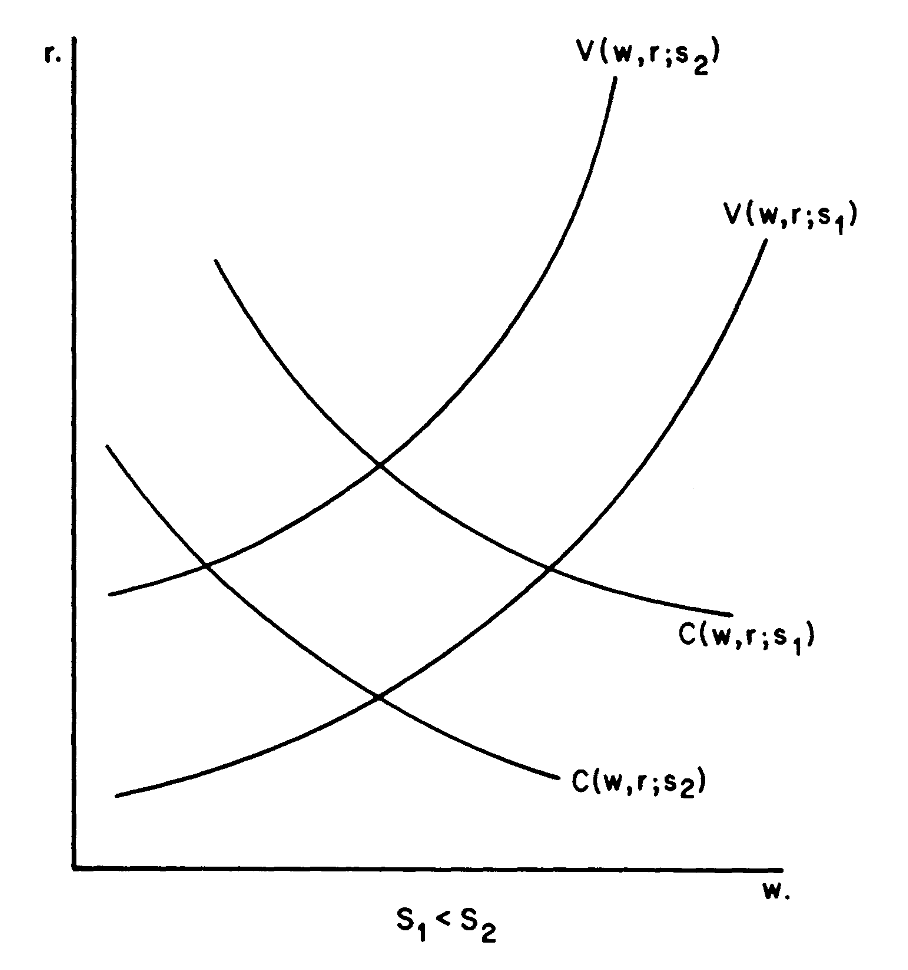
\includegraphics[width=0.5\textwidth]{image/Roback1986Equilibrium.png}

The following equations represent the effects of changes in $s$ on $w$ and $r$:

\begin{equation}
\begin{split}
&\frac{dw}{ds} = \frac{1}{\triangle}[-V_s C_r + C_s V_r] < 0
\\&\frac{dr}{ds} = \frac{1}{\triangle}[-V_wC_s + V_sC_w] \lessgtr 0
\end{split}
\label{roback equilibrium}
\end{equation}
where $\triangle = V_w C_r - V_r C_w = \frac{L(s) V_w}{X}>0$, $L(s)$ is the total land available at location $s$. Subscripts denote partial derivatives.



The equations show that in locations with more amenities, wages are lower, while the change in rents is ambiguous.

\subsection{Applications} % (fold)
\label{sub:applications}

The model has several potential applications.

\textbf{Imputing implicit prices}

Now the equations \ref{roback equilibrium} can be used to derive the implicit price of the amenity, $s$.

\begin{equation}
  p^*_s \equiv \frac{V_s}{V_w}=l^c \frac{dr}{ds}-\frac{dw}{ds}
\end{equation}

\begin{equation}
  p^*_sN(\tilde s)+[-C_s X(\tilde s)]=\frac{dr}{ds}L(\tilde s)
\end{equation}

where $k_l$ is the share of land in the consumer's budget.

Computing quality of life indices: The implicit prices of different city characteristics can be used as weights to compute a quality of life index.

Cost-benefit analysis: The model can be used to calculate the aggregate willingness to pay for changes in environmental variables.

Adjusting national income accounts: The model can help adjust GNP accounts to reflect changes in quality of life.

\textbf{The Housing Market and Other Nontraded Goods}

The model can be extended to include a nontraded goods sector, such as housing. This requires adding the vector of nontraded goods, $y$, to the utility function and introducing a nontraded-goods sector with unit cost function $G(w, r; s)$.

The extended model yields a more complex equation for the price-amenity gradient:

$\frac{dp}{ds} = \frac{1}{A^*}[+V_s(-GC_r + G_rC) - C_s(G_rV_w) + G_s(V_wC_r)]$, (9)

where $A^* = V_wC_r - V_p(C_wG_r - C_rG_w) > 0$.

This extended model shows that predictions about housing prices are more complex than predictions about land prices.

The amenity effects and the productivity effects can be derived as:

$p^* = \frac{V_s}{V_w}\frac{dp}{ds} - \frac{dw}{ds}$

$C_s = -\theta_l^f\frac{dw}{ds} + \theta_r^f\frac{dr}{ds}$

$G_s = \frac{dp}{ds} - \theta_w^g\frac{dw}{ds} - \theta_r^g\frac{dr}{ds}$

where $\theta_i^j$ is the share of factor $i$ in the cost of producing good $j$.

This expanded model illustrates how the applications of the basic model can be extended to include nontraded goods.
% subsection subsection_name (end)The Housing Market and Other Nontraded Goods

%
%
%
\part{Others}
\section{Krugman 1991} % (fold)
\label{sec:krugman_1991}
\subsection{Dixit and Stiglitz 1977} % (fold)
\label{sub:dixit_and_stiglitz}
For better intuition of krugman's Core-Periphery model, a quick read about Dixit and Stiglitz is neccesary. Before this iconic paper of theirs, neoclassical economics tended to describe economy as perfect competitive and constant return to scale. Dixit and Stiglitz used CES utility function and non-convex production function to build a monopolistic competitive model with increasing return. However this masterpiece of model pictures a world of teleporters, who does not care the distance or time delay. Krugman stepped in and filled the hole with his unique ideas. Therefore Krugman's Core-Periphery model is sometimes called the Dixit-Stiglitz-Krugman model (DSK model).
% subsection dixit_and_stiglitz (end)
\subsection{Assumptions} % (fold)
\label{sub:assumptions}
\textbf{Two regions}

Region 1 and region 2. Without furthur specified, they are identical at the begenning.

\textbf{Two sectors}
\begin{itemize}
  \item Agricultural production, constant return to land
  \item Industrial production, increasing return
\end{itemize}

\textbf{Individual's utility production}
\begin{equation}
  U=C^\mu_M C^{1-\mu}_A
\end{equation}
$\mu > 1$ is the share of expenditure, $C_M$ is aggregate consumption of manufactured goods, $C_A$ is of agricultural.

\textbf{Competitive monopolistic}

Another important thing is that the manufactures are distinguishly different. To illustrate so, the demand of $C_M$ is CES form.
\begin{equation}
  C_M=[\sum\limits_{i=1}^{N}C_i^{\frac{\sigma-1}{\sigma}}]^{\frac{\sigma}{\sigma-1}}
\end{equation}

\textbf{Work force}

The society has one unit of labor force.

$\mu$ represents mobile workers in industry and has the distribution of 
\begin{equation}
  L_1+L_2=\mu \label{worker distribution}
\end{equation}

$1-\mu$ represents immobile peasants in agriculture and has the equal distribution of 
\begin{equation}
  \frac{1-\mu}{2}+\frac{1-\mu}{2}=1-\mu \label{peasant distribution}
\end{equation}

\textbf{Production}
\begin{equation}
  L_{M_i}=\alpha+\beta x_i
\end{equation}
$L_{M_i}$ is the labor used in producing manufacture $i$, and $x_i$ is the output.

\textbf{Transportation cost}

For agricultural goods, the transportation is costless. And for manufacture goods, we take Samuelson's Iceburg approach. Only $\tau$ percent of goods will arrive after transportation. (This also implies the transportation cost happens during the process of transportation)

% subsection assumptions (end)

\subsection{Firm behavior} % (fold)
\label{sub:firm_behavior}
\textbf{Price setting}

In a monopolistic competitive market, the optimal price setting strategy of a firm is 
\begin{equation}
  p_1 = \underbrace{(\frac{\sigma}{\sigma-1})}_{\text{markup}}\underbrace{\beta w_1}_{\text{marginal cost}}
  \label{firm price setting}
\end{equation}
and similarly 
\begin{equation}
  p_2=\frac{\sigma}{\sigma-1}\beta w_2
\end{equation}
The relative price is 
\begin{equation}
  \frac{p_1}{p_2}=\frac{w_1}{w_2}
\end{equation}

\textbf{Number of goods}

Assuming there is free entry into the market, profit must be zero. Applying equation \ref{firm price setting}, we could
$$
\begin{aligned}  
&p_1 x_1 - (\beta x_1 +\alpha)w_1=0
\\\Rightarrow & (p_1-\beta w_1)x_1=\alpha w_1
\\\Rightarrow & x_1=\frac{\alpha w}{p_1-\beta w_1}=\frac{\alpha}{\frac{p_1}{w_1}-\beta}
\end{aligned}$$
\begin{equation}
  \Rightarrow x_1=x_2=\frac{\alpha(\sigma-1)}{\beta} \label{output behavior}
\end{equation}

\textbf{Number of firms}

It all implies that the number of firms in each region is proportional to the workers in each region
\begin{equation}
  \frac{n_1}{n_2}=\frac{L_1}{L_2}
\end{equation}

% subsection firm_behavior (end)
\subsection{Short run equilibrium} % (fold)
\label{sub:short_run_equilibrium}

Let $c_{ij}$ be the consumption of region $i$ on the goods manufactured in region $j$

In short run equilibrium, 
\begin{equation}
  \frac{c_{11}}{c_{12}}=(\frac{p_1}{\frac{p_2}{\tau}})^{-\tau}=(\frac{\tau w_1}{w_2})^{-\tau}
\end{equation}

Let $z_{ij}$ be the ratio of region $i$ expenditure on local manufactures that on manufactures from region $j$

\begin{equation}
  z_{11}=(\frac{n_1}{n_2})(\frac{p_1 \tau}{p2})(\frac{c_{11}}{c_{12}})=(\frac{c_1}{c_2})(\frac{w_1 \tau}{w_2})^{-(\sigma-1)} \label{z11}
\end{equation}

and similiarly
\begin{equation}
  z_{12}=(\frac{L_1}{L_2})(\frac{w_1 \tau}{w_2})^{-(\sigma-1)}
\end{equation}

and income of workers in the two regions are 
\begin{align}
  w_1 L_1 =\mu[(\frac{z_{11}}{1+z_{11}})Y_1+(\frac{z_{12}}{1+z_{12}})Y_2]
  \\
  w_2 L_2 =\mu[(\frac{1}{1+z_{11}})Y_1+(\frac{1}{1+z_{12}})Y_2]
\end{align}

Recall that a region is consisted of workers and peasants, who hold up to $\frac{1-\mu}{2}$. Let the income of peasants be unit free, the total income of households in a region is 
\begin{align}
Y_1 = \frac{1-\mu}{2}+w_1 L_1 \label{income of region 1}
\\Y_2 = \frac{1-\mu}{2}+w_2 L_2 \label{income of region 2}
\end{align}

Now the equations \ref{z11}-\ref{income of region 2} are sufficient to determine the equilibrium, that is a sequence of $\{w_1,w_2,z_1,z_2,Y_1,Y_2\}$.

% subsection short_run_equilibrium (end)
\subsection{Long run equilibrium} % (fold)
\label{sub:long_run_equilibrium}

Recall by definition in equation \ref{worker distribution}, the worker supply is $L_1 +L_2 =\mu$. Let $f_i$ be the share ratio of worker supply of region $i$, that is 
\begin{equation}
  f_i = \frac{L_i}{\mu} \label{worker share ratio}
\end{equation}

The real price index of manufacture goods in region 1 is 
\begin{equation}
  P_1 = [f w_1^{-(\sigma-1)}+(1-f)(\frac{w_2}{\tau})^{-(\sigma-1)}]^{-\frac{1}{\sigma-1}} \label{true price index 1}
\end{equation}
and in region 2. the households face the price index
\begin{equation}
  P_2 = [f (\frac{w_1}{\tau})^{-(\sigma-1)}+(1-f)(w_2)^{-(\sigma-1)}]^{-\frac{1}{\sigma-1}} \label{true price index 2}
\end{equation}

Now according to equation \ref{true price index 1} and \ref{true price index 2}, when $w_1 =w_2 $, a shift to region 1 will lower $P_1$ and raise $P_2$. This is called price index effect.

Let $\omega_i$ be real wage rate in regino $i$, we have 
\begin{align}
\omega_1 = w_1 P_1^{-\mu}\\
\omega_2 = w_2 P_2^{-\mu}
\end{align}
When $\omega_1=\omega_2$, $\frac{\omega_1}{\omega_2}$ increases as $f$ increases. This is exactly price index effect.


Symmetric Case: If $f = 0.5$, that is when the two regions have equal number  of workers, they offer equal real wage rates, $\frac{\omega1}{\omega2} = 1$.

Regional Convergence: If $\frac{\omega1}{\omega2}$ decreases with $f$, i.e., the relative real wage is lower when work force is larger, then workers tend to migrate out of the region  with larger worker force. (One force: degree of competition for local peasant market)

Regional Divergence: If $\frac{\omega1}{\omega2}$ increases with $f$, i.e., the relative real wage is  higher when work force is larger, then workers tend to migrate into the region  with larger worker force. (Two forces: home market effect and price index  effect)

% subsection long_run_equilibrium (end)
\subsection{Comments on how Krugman tries to explain the immigration} % (fold)
\label{sub:comments_on_how_krugman_tries_to_explain_the_immigration}

He developed the core-periphery model, which explains how some regions become economically dominant (the "core") while others lag behind (the "periphery"), based on the interplay between economies of scale and transport costs.

Krugman thinks real life friction like transportation cost is the key reason why externality promoting agglomeration economy occurs. And because of so, the workers tend to join in a core region to enjoy lower price. Krugman's NEG model is best for explaination that people join the big urban cities.

\textbf{Further development}
Krugman's CP model is classical, yet lacks the availablity of analytical solution. It also doges the existence of transportation sector by using Samuelson's iceburg theory.

\begin{itemize}
  \item Fujita et al., 2000, 
  \item Ottaviano et al., 2002, Agglomeration and Trade Revisited. He developed a new linearized economic geography model, from which analytical solutions can be obtained.
  \item Behrens et al., 2009, Industry Location and Welfare When Transport Costs Are Endogenous. He endogenized transportation cost.
  \item Z. Xu and S. Li, 2009, The Effects of Inter-regional Migration on Regional Disparities
\end{itemize}


% subsection comments_on_how_krugman_tries_to_explain_the_immigration (end)
% section krugman_1991 (end)
% -------------------------------------------------------
\section{Fujita 2000} % (fold)
\label{sec:fujita_2000}




% -------------------------------------------------------
% -------------------------------------------------------
% -------------------------------------------------------
\part{Conclusion}
\section{Comparison} % (fold)
\label{sec:comparison}
For comparison, see the chart below
\begin{table}[h]
    \centering
    \begin{tabular}{ccccc}
         \textbf{Model}&  \textbf{Sectors}&  \textbf{Reason of migration}& \\
         Tiebout&  Different public goods and tax rates&   Different preferences& \\
         Todaro&  Dual economy&   Rational expection of wage gap& \\
         Krugman&  Core city and periphery city&   Tranportation fee& \\
         Push-pull&  Start and destination&   All kinds of reasons& \\
    \end{tabular}
    \caption{Comparison of four models}
    \label{tab:comparison}
\end{table}

It is wild but reasonable to say:
\begin{itemize}
  \item Push-pull model covers Tiebout model. Voting with your feet is rooted in people's different preferences. Public goods and tax rates of both ends can be seen as push and pull factors.
  \item Krugman's core-periphery model emphasizes the relationship of two mostly identical cities, whereas Todaro's model emphasizes the relationship of a rural area and an urban area.
  \item All models above can be empirically tested by econometrics.
\end{itemize}



% section comparison (end)
% -------------------------------------------------------
\end{document}